\documentclass[12pt]{article}
\usepackage[utf8]{inputenc}
\usepackage[T1]{fontenc}
\usepackage{setspace}
\usepackage{a4}
\usepackage{amssymb,amsmath,amsthm,latexsym,amsfonts}
\usepackage{array}
\usepackage[numbers]{natbib}
\bibliographystyle{plainnat}
\usepackage{float}
\usepackage[nottoc]{tocbibind}
\setlength{\parindent}{1.0cm}
\setlength{\evensidemargin}{0.0cm}
\setlength{\oddsidemargin}{0.0cm}
\setlength{\topmargin}{0.0cm}
\textwidth 17cm
\textheight 20cm
\onehalfspacing

\usepackage{microtype}
\usepackage{tablefootnote}
\usepackage{threeparttable}
\usepackage{booktabs}
\usepackage{caption}
\captionsetup{justification=raggedright,singlelinecheck=false,font=footnotesize}
\captionsetup[table]{labelsep=newline}
\captionsetup[figure]{labelsep=period}
\usepackage{bm}
\usepackage{stfloats}
\usepackage{mathrsfs}
\usepackage{tabularx}
\usepackage{multirow}
\usepackage{enumitem}
\usepackage{textcomp}
\usepackage{subcaption}
\captionsetup[subfigure]{font=footnotesize}
\usepackage{adjustbox}
\usepackage{graphicx}
\usepackage{listings}
\usepackage{xcolor}
\usepackage{multicol}
\usepackage{longtable}
\usepackage{algorithm,algorithmic}
\usepackage{etoolbox}
\usepackage{amsthm,xpatch}
\usepackage[hidelinks]{hyperref}

\definecolor{dkgreen}{rgb}{0,0.6,0}
\definecolor{gray}{rgb}{0.5,0.5,0.5}
\definecolor{mauve}{rgb}{0.58,0,0.82}
\lstset{frame=tb,
  language=Python,
  aboveskip=3mm,
  belowskip=3mm,
  showstringspaces=false,
  columns=flexible,
  basicstyle={\small\ttfamily},
  numbers=none,
  numberstyle=\tiny\color{gray},
  keywordstyle=\color{blue},
  commentstyle=\color{dkgreen},
  stringstyle=\color{mauve},
  breaklines=true,
  breakatwhitespace=true,
}

\newtheorem{definition}{Definition}
\newtheorem{lemma}{Lemma}
\xpatchcmd{\@thm}{\fontseries\mddefault\upshape}{}{}{}
\newcommand*{\comb}[2]{{}^{#1}C_{#2}}
\newcommand{\RNum}[1]{\lowercase\expandafter{\romannumeral #1\relax}}
\makeatletter
\@dblfptop 0pt
\makeatother

\begin{document}

\begin{titlepage}
\doublespacing

\begin{center}
{\large \textbf{Mini Project Report}}\\[0.3cm]
{\large \textbf{on}}\\[0.4cm]
{\Large \textbf{Medical Insurance Claim Fraud Detection: \\ Multi-Paradigm Machine Learning, Deep Learning, \\ Agentic XAI, and Verified Dual-Path Deployment}}
\end{center}

\vspace{0.5cm}

{\small
\begin{center}
Submitted by \\[0.2cm]
{\large \textbf{B. Varshith (23BDS011)}}\\
{\large \textbf{J. Ganesh Kumar Reddy (23BDS024)}}\\
{\large \textbf{M. Jagadeeswar (23BDS033)}}\\[0.4cm]
Under the guidance of \\[0.2cm]
{\large \textbf{Prof. Ramesh Athe}}\\
\textbf{Department of Computer Science and Engineering}
\end{center}
}

\begin{figure}[h]
\begin{center}

\includegraphics[height=.80in]{iiitdwd_logo.png}
\end{center}
\end{figure}

\begin{center}
{\small\textbf{DEPARTMENT OF COMPUTER SCIENCE AND ENGINEERING}}\\
{\small\textbf{INDIAN INSTITUTE OF INFORMATION TECHNOLOGY DHARWAD}}\\
11/11/2026
\end{center}
\end{titlepage}

\newpage
\thispagestyle{empty}
\clearpage
\thispagestyle{empty}
\phantom{a}
\newpage
\thispagestyle{empty}

\begin{center}
	\emph{\huge{Certificate}}\\[2.0cm]
\end{center}
\normalsize This is to certify that the project, entitled \textbf{Medical Insurance Claim Fraud Detection: Multi-Paradigm Machine Learning, Deep Learning, Agentic XAI, and Verified Dual-Path Deployment}, is a bonafide record of the Mini Project coursework presented by the students whose names are given below during Academic Year 2025--2026 in partial fulfilment of the requirements of the degree of Bachelor of Technology in Computer Science and Engineering (with Data Science and Artificial Intelligence cohort).\\[1.0cm]

\begin{table}[h]
	\centering
	\begin{tabular}{lr}
		Roll No & Names of Students \\ \hline
		\\
		23BDS011 & B. Varshith \\
		23BDS024 & J. Ganesh Kumar Reddy \\
		23BDS033 & M. Jagadeeswar \\
	\end{tabular}
\end{table}

\vfill

\begin{flushright}
	Prof. Ramesh Athe\\
	(Project Supervisor)\\[1.5cm]
\end{flushright}

\newpage
\pagenumbering{roman}
\setcounter{page}{1}
\begin{abstract}
Healthcare insurance fraud imposes substantial financial losses on insurers and beneficiaries while demanding low false-alarm triage and transparent audit justification for human investigators. On a verified corpus of 4,500 medical insurance claims (270 fraudulent, 6.00\% prevalence), this project presents a unified, leakage-governed fraud intelligence platform uniting three complementary AI approaches—Classical Machine Learning (5 algorithms), PyTorch Deep Learning (4 supervised architectures plus 1 unsupervised Autoencoder ablation), and Agentic AI with Explainability (XAI) and Gemini conversational assistance—deployed across both a three-tier React/Node/FastAPI application (Track A, 29 features) and a controlled browser-native benchmark lab (Track B, 4 experimental protocols over 32 runs). A rigorous dataset audit exposed two critical pitfalls: an upstream \texttt{Cluster} variable acting as a leaky label proxy (concentrating 267 of 270 frauds in Cluster 1) and an amount boundary separating all positives at \texttt{ClaimAmount} $\ge 7,465.07$. Under the leakage-free \texttt{Intake} contract (28 features excluding \texttt{Cluster}) and strict validation-$F_1$ thresholding, Random Forest and XGBoost achieve 1.0000 test Average Precision (PR-AUC), with Random Forest attaining $F_1 = 0.9873$ (0 false positives, 1 missed fraud) and maintaining $F_1 = 1.0000$ under chronological future testing ($\ge$ 2024-03-11). Among deep learners on the 29-feature contract, TabTransformer leads with 0.9911 PR-AUC ($F_1 = 0.8989$), followed by CNN1D (0.9882), ResidualMLP (0.9561), and MLP (0.9538), whereas an unsupervised Autoencoder trained solely on legitimate claims yields a documented negative result (0.0523 PR-AUC, 0.0299 $F_1$). Finally, exported browser weights match Python reference execution across 10,800 score evaluations within $4.42 \times 10^{-7}$ maximum absolute difference with zero decision flips, while the Node/Express and React system exposes all 10 ML/DL endpoints, an interactive Gemini co-pilot, and a documented roadmap bridging deterministic agentic routes to live multi-agent RAG execution.
\end{abstract}

\newpage
\tableofcontents
\newpage
\listoffigures
\newpage
\listoftables

\newpage
\thispagestyle{empty}
\clearpage
\thispagestyle{empty}
\phantom{a}
\newpage

\pagenumbering{arabic}
\section{Introduction}

Healthcare insurance billing systems process high-volume outpatient, inpatient, routine, and emergency claims daily, creating severe exposure to upcoding, duplicate billing, phantom procedures, and eligibility abuse \cite{dupreez2025fraud, bauder2017medicare}. Automating fraud screening requires resolving five coupled technical tensions rather than merely fitting an off-the-shelf binary classifier: (1) severe positive-class scarcity (only 6.00\% positive prevalence in our operational corpus), (2) vulnerability to upstream feature leakage and single-feature shortcuts \cite{kaufman2012leakage, geirhos2020shortcut}, (3) divergence between inductive biases of tree ensembles versus neural networks on medium-sized tabular tables \cite{grinsztajn2022tree}, (4) uncalibrated threshold drift when transitioning to forward-in-time claim arrivals, and (5) Special Investigation Unit (SIU) demands for human-understandable attribution rather than opaque scalar probabilities \cite{lundberg2017unified}.

\subsection{Problem Statement and Research Objectives}
Given raw structured insurance records $\mathcal{D} = \{(\mathbf{r}_i, y_i)\}_{i=1}^{4500}$ with 19 columns and binary target $y_i = \mathbb{I}(\text{ClaimLegitimacy}_i = \text{Fraud})$, our goal is to engineer an auditable, end-to-end decision support system achieving the following objectives:
\begin{enumerate}[label=\arabic*.]
    \item \textbf{Leakage & Distributional Governance:} Audit every column in \texttt{Health Insurance Fraud Claims.xlsx} for identifier memorization, upstream clustering proxies (\texttt{Cluster}), and single-variable separation (\texttt{ClaimAmount}), constructing explicit experimental ablation contracts.
    \item \textbf{Multi-Paradigm Model Evaluation:} Implement, tune, and benchmark 10 distinct models spanning Classical Machine Learning (\textbf{Approach 1}), Supervised and Unsupervised Deep Learning (\textbf{Approach 2}), and Agentic/LLM Triage (\textbf{Approach 3}).
    \item \textbf{Imbalance-Aware Protocol:} Prioritize Precision-Recall Area Under Curve (PR-AUC / AP) over optimistic accuracy or ROC-AUC \cite{saito2015precision}, calibrate binary operating thresholds $\tau^*$ solely on held-out validation folds, and quantify uncertainty via stratified bootstrap resampling.
    \item \textbf{Dual-Path Engineering & Parity:} Deliver both (i) a three-tier React/Node/FastAPI application serving all 10 ML/DL endpoints, Gemini 2.0 Flash claim chat, and an Agentic pipeline view (\textbf{Track A}), and (ii) a pure-JavaScript browser Claim Fraud Lab verified against Python reference outputs within numerical tolerance (\textbf{Track B}).
\end{enumerate}

\subsection{Key Project Contributions and Team Attribution}
The platform was architected and built collaboratively at the Department of Computer Science and Engineering, IIIT Dharwad under the guidance of Prof. Ramesh Athe:
\begin{itemize}
    \item \textbf{Approach 1 & Leakage/Parity Benchmark Lab (J. Ganesh Kumar Reddy, 23BDS024):} Comprehensive exploratory audit, 5 classical ML pipelines, 4-scenario sensitivity/temporal benchmark framework (\texttt{submission/}), bootstrap analysis, error forensics, and pure-JS weight exporter.
    \item \textbf{Approach 2 & Full-Stack Integration (M. Jagadeeswar, 23BDS033):} Five PyTorch deep learning architectures (\texttt{MLP}, \texttt{ResidualMLP}, \texttt{CNN1D}, \texttt{TabTransformer}, and \texttt{Autoencoder}), unified FastAPI \texttt{ml-service} (\texttt{:8000}), Node.js API proxying (\texttt{:3000}), and React ML/DL workbenches (\texttt{:5173}).
    \item \textbf{Approach 3 Agentic Triage, XAI & Gemini Co-Pilot (B. Varshith, 23BDS011):} Six-role frontend agent pipeline UI (\texttt{AgenticDashboard.tsx}), Express \texttt{AgenticEnsemble-v1} handler, SHA-256 cryptographic XAI log utility (\texttt{Approach-3-Agentic-AI}), and live Google Gemini \texttt{/api/chat} assistant.
\end{itemize}

\newpage
\section{Related Work}

\subsection{Machine Learning for Healthcare Claims Fraud Detection}
Systematic reviews confirm the primacy of supervised ensemble modeling in healthcare claim screening. du Preez et al.\ \cite{dupreez2025fraud} reviewed 137 primary ML healthcare fraud publications, concluding that gradient boosted decision trees and Random Forests \cite{breiman2001random, chen2016xgboost, ke2017lightgbm} remain dominant on structured tabular claim data while noting widespread gaps in chronological evaluation and cost-sensitive thresholding. Bauder and Khoshgoftaar \cite{bauder2017medicare} analyzed Medicare Part B billing records under extreme class imbalance, demonstrating substantial sensitivity advantages of random forests and boosting over linear regression and support-vector networks \cite{cortes1995support}. Kapadiya et al.\ \cite{kapadiya2022blockchain} further advocated combining predictive AI engines with tamper-evident ledger or cryptographic audit trails to guarantee investigator accountability across insurer workflows.

\subsection{Deep Learning for Tabular Data and Unsupervised Anomaly Modeling}
Applying deep neural networks to medical claims presents distinct inductive-bias challenges. Johnson and Khoshgoftaar \cite{johnson2019medicare} established that tabular neural models on Medicare datasets require weighted loss formulations or sampling strategies such as SMOTE \cite{chawla2002smote} to avoid majority-class collapse. Subsequent tabular architectures incorporated residual identity skip connections \cite{he2016deep, gorishniy2021revisiting} and multi-head self-attention across discrete embeddings in \textbf{TabTransformer} \cite{huang2020tabtransformer}. However, Grinsztajn et al.\ \cite{grinsztajn2022tree} demonstrated across 45 medium-sized ($\sim$10K sample) benchmarks that tree-based ensembles routinely outperform neural architectures when informative thresholds are axis-aligned and uninformative covariates coexist—a phenomenon directly observed in our \texttt{Intake} ablation. For unlabeled regimes, Sakurada and Yairi \cite{sakurada2014anomaly} and Chalapathy and Chawla \cite{chalapathy2019deep} showed autoencoders detect manifold-breaking anomalies via reconstruction error, yet warn of failure when anomalous examples lie embedded within high-density legitimate feature bounds.

\subsection{Imbalanced Evaluation, Leakage Governance, and Shortcut Learning}
When fraud prevalence is $6\%$, Saito and Rehmsmeier \cite{saito2015precision} proved that ROC-AUC becomes overly optimistic because false positives are diluted by a large negative denominator, making Precision-Recall plots and Average Precision (PR-AUC) mandatory for operational assessment. Simultaneously, Kaufman et al.\ \cite{kaufman2012leakage} formalized training-serving leakage from post-hoc target proxies, and Geirhos et al.\ \cite{geirhos2020shortcut} documented how high i.i.d.\ test accuracy masks fragile single-feature shortcuts. Our controlled \texttt{Intake} and \texttt{No-Amount} ablations operationalize both safeguards explicitly.

\subsection{Explainable AI (XAI), RAG, and Agentic Insurance Triage}
Regulatory claim auditing requires local feature explanations such as SHAP \cite{lundberg2017unified} alongside verifiable policy citations enabled by Retrieval-Augmented Generation (RAG) \cite{lewis2020retrieval}. Emerging agentic AI claim pipelines decompose review into intake validation, code analysis, quantitative fraud scoring, and investigator report synthesis—motivating Approach 3's separation between UI visualization, XAI cryptographic hashing, live Gemini chat synthesis, and real-time FastAPI model endpoints.

\newpage
\section{Data and Methods}

\subsection{Audited Dataset Characterization and Leakage Discovery}
All experiments draw from a single immutable workbook, \texttt{Health Insurance Fraud Claims.xlsx} (SHA-256 \texttt{952b6e23...614b6a45}), containing $N = 4,500$ claims across 19 columns spanning 731 days (\texttt{2022-07-09} to \texttt{2024-07-08}) with zero missing entries and zero duplicate rows. Exactly $270$ claims are labeled Fraud ($6.00\%$) and $4,230$ Legitimate ($94.00\%$). Six identifier or near-unique code fields (\texttt{ClaimID}: 4,500 unique; \texttt{PatientID}: 4,500; \texttt{ProviderID}: 4,500; \texttt{DiagnosisCode}: 4,495; \texttt{ProcedureCode}: 4,495; \texttt{ProviderLocation}: 3,876) were excluded from supervised matrices to prevent record memorization.

Crucially, exploratory audit uncovered two structural hazards visualized in Fig.~\ref{fig:audit}:
\begin{enumerate}
    \item \textbf{Upstream \texttt{Cluster} Leakage:} Feature \texttt{Cluster} $\in \{0,1,2,3\}$ concentrates \textbf{267 of 270 frauds (98.89\%)} inside Cluster 1 ($267/1,100 = 24.27\%$ rate), whereas Clusters 0 and 2 contain $0$ frauds ($0/1,144$ and $0/1,104$) and Cluster 3 contains only $3/1,152$ ($0.26\%$).
    \item \textbf{Single-Feature Amount Threshold:} Fraudulent claims occur exclusively at \texttt{ClaimAmount} $\in [7,465.07, 9,978.43]$ (mean $8,733.57$), whereas legitimate claims span $[100.12, 9,997.20]$ (mean $4,776.80$).
\end{enumerate}

\begin{figure}[H]
\centering
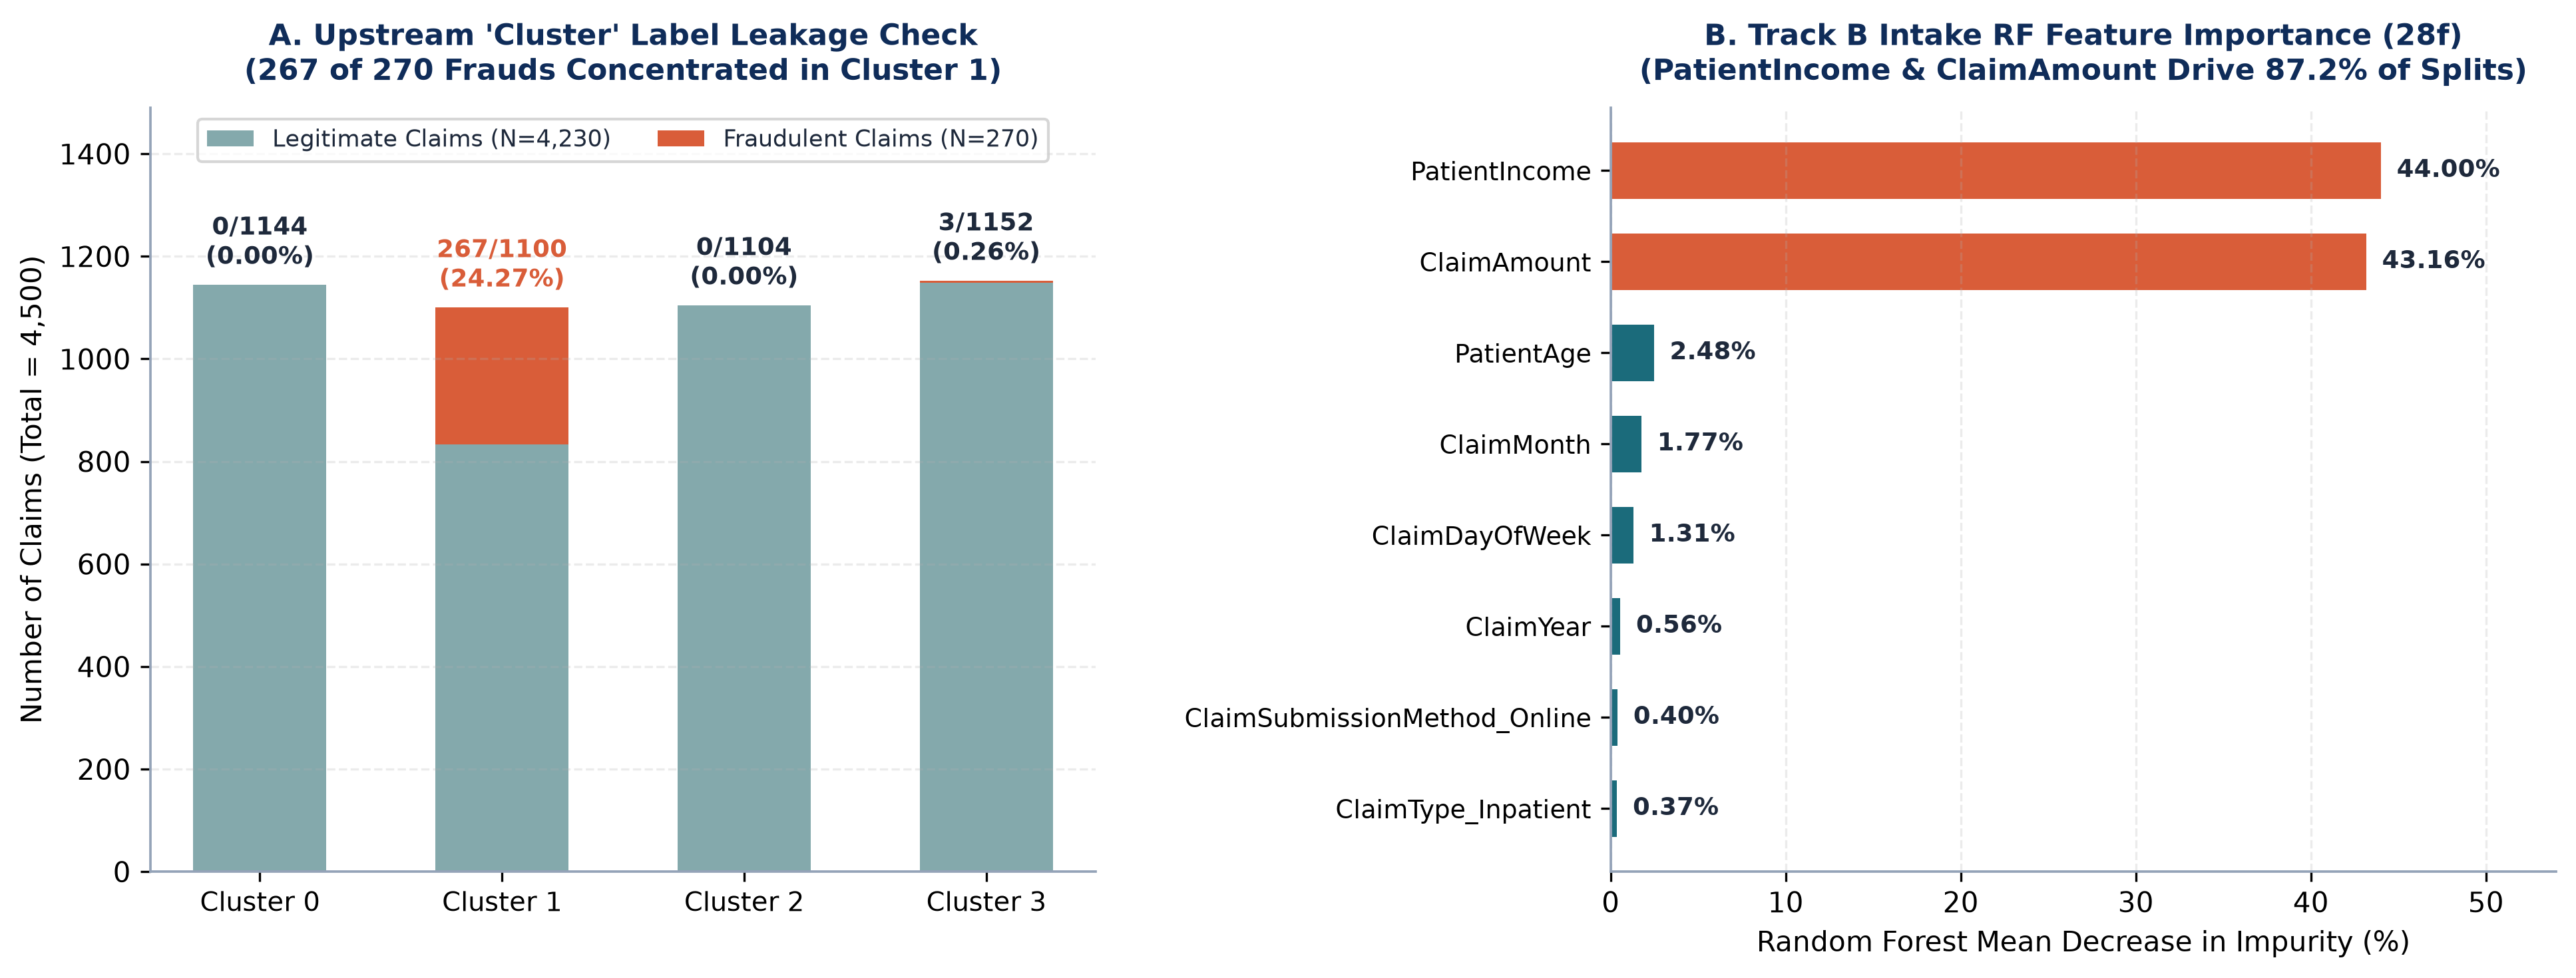
\includegraphics[width=\textwidth]{figures/fig2_data_audit_shortcuts.png}
\caption{Exploratory data audit: (A) upstream \texttt{Cluster} concentrates 98.89\% of frauds in Cluster 1; (B) without \texttt{Cluster}, Random Forest relies primarily on \texttt{PatientIncome} (44.00\%) and \texttt{ClaimAmount} (43.16\%).}
\label{fig:audit}
\end{figure}

\subsection{Mathematical Formulation and Feature Contracts}
For each claim $\mathbf{r}_i$, calendar date decomposes into \texttt{ClaimYear}, \texttt{ClaimMonth}, and \texttt{ClaimDayOfWeek}. A scikit-learn \texttt{ColumnTransformer} fits \texttt{StandardScaler} on continuous features and \texttt{OneHotEncoder(handle\_unknown="ignore")} on 7 categorical attributes (\texttt{PatientGender}, \texttt{ProviderSpecialty}, \texttt{ClaimStatus}, \texttt{PatientMaritalStatus}, \texttt{PatientEmploymentStatus}, \texttt{ClaimType}, \texttt{ClaimSubmissionMethod}) \emph{strictly on the training split}. We define four controlled contracts summarized in Table~\ref{tab:contracts}.

\begin{table}[H]
\centering
\caption{Controlled Experimental Feature and Split Contracts (Track A vs. Track B)}
\label{tab:contracts}
\small
\begin{tabular}{@{}llccp{4.9cm}@{}}
\toprule
Contract & Split Policy & Dim ($d_s$) & Train / Val / Test (Positives) & Experimental Objective \\ \midrule
\textbf{Baseline} (Track A/B) & Stratified Seed 42 & 29 & 3,150 (189) / 675 (41) / 675 (40) & Canonical API contract retaining \texttt{Cluster}. \\
\textbf{Intake} (Track B) & Stratified Seed 42 & 28 & 3,150 (189) / 675 (41) / 675 (40) & Deployment-realistic protocol removing \texttt{Cluster}. \\
\textbf{No-Amount} (Track B) & Stratified Seed 42 & 27 & 3,150 (189) / 675 (41) / 675 (40) & Shortcut stress test dropping \texttt{Cluster} \& \texttt{ClaimAmount}. \\
\textbf{Temporal} (Track B) & Chronological Date & 28 & 3,152 (199) / 677 (34) / 671 (37) & Future rollout split (Test $\ge$ \texttt{2024-03-11}). \\ \bottomrule
\end{tabular}
\end{table}

All supervised neural networks minimize weighted binary cross-entropy to counter the $15.67:1$ legitimate-to-fraud ratio:
\begin{equation}
\mathcal{L}_{\text{wBCE}}(\theta) = -\frac{1}{|\mathcal{D}_{\text{train}}|}\sum_{i \in \mathcal{D}_{\text{train}}} \left[ w^+ y_i \log \sigma(z_i) + (1-y_i)\log\big(1-\sigma(z_i)\big) \right], \quad w^+ = \frac{N_{-,\text{train}}}{N_{+,\text{train}}},
\end{equation}
using AdamW regularization and validation PR-AUC early stopping. Decision thresholds $\tau^*$ are fixed either at canonical $0.50$ (Track A API compatibility) or optimized on the held-out validation fold $\tau^* = \arg\max_{\tau} F_1(\mathbf{y}_{\text{val}}, \mathbb{I}(\hat{\mathbf{p}}_{\text{val}} \ge \tau))$ prior to frozen test evaluation (Track B). Unsupervised \texttt{Autoencoder} minimizes legitimate-only MSE $\|\mathbf{x}_i - D_\psi(E_\psi(\mathbf{x}_i))\|_2^2$ with anomaly cutoff selected at the 95th percentile of validation errors ($\tau_{\text{AE}} = 0.128588$).

\subsection{Three-Approach Architecture and Dual-Path Engineering}
Figure~\ref{fig:arch} illustrates the complete platform integrating Approaches 1--3 across two synchronized deployment paths:
\begin{itemize}
    \item \textbf{Approach 1 — Classical Machine Learning:} Five models covering generalized linear separation (\texttt{LogisticRegression}, balanced L2), bagging trees (\texttt{RandomForest}, 200 trees, balanced), boosting ensembles (\texttt{XGBoost}, \texttt{scale\_pos\_weight}=15.67, \texttt{eval\_metric=aucpr}; \texttt{HistGradientBoostingClassifier}, 200 iterations), and kernel margins (\texttt{SVM}, RBF with Platt probability scaling).
    \item \textbf{Approach 2 — Deep Learning (PyTorch):} Five distinct neural paradigms trained in \texttt{Approch-2-DL/}: \texttt{FraudMLP} ($29 \to 64 \to 32 \to 1$ with BatchNorm/Dropout), \texttt{ResidualMLP} (skip-connected residual blocks), \texttt{FraudCNN1D} (1D convolutions treating aligned features as a sequence), \texttt{TabTransformer} (contextual multi-head self-attention across discrete embeddings fused with continuous projections), and \texttt{Autoencoder} ($29 \to 16 \to 8 \to 16 \to 29$ trained on $y=0$ only).
    \item \textbf{Approach 3 — Agentic AI, XAI & Conversational Co-Pilot:} As detailed in Fig.~\ref{fig:agentic}, the React frontend (\texttt{AgenticDashboard.tsx}) presents a six-role triage pipeline alongside an interactive Gemini 2.0 Flash co-pilot (\texttt{POST /api/chat}), while the Node/Express gateway (\texttt{POST /agentic/predict}) executes \texttt{AgenticEnsemble-v1} emitting a four-stage trace (\texttt{ingestion}, \texttt{validation}, \texttt{risk-scorer}, \texttt{xai-explainer}). Standalone \texttt{Approach-3-Agentic-AI} provides \texttt{XAIExplainer} magnitude-normalized feature attributions and SHA-256 tamper-evident audit hashes. We transparently document that live FastAPI checkpoint chaining, OCR ingestion, and policy RAG remain next-phase integrations atop the active deterministic risk handler.
    \item \textbf{Path A (3-Tier Full-Stack) vs. Path B (Browser Parity Lab):} Path A links React (\texttt{:5173}) $\to$ Express (\texttt{:3000}) $\to$ FastAPI (\texttt{:8000}) serving all 10 ML/DL checkpoints. Path B (\texttt{submission/}) compiles sklearn scalars/OHE, tree splits, RBF support vectors, and PyTorch tensors into static JSON for pure-JS browser inference (\texttt{:8080}).
\end{itemize}

\begin{figure}[H]
\centering
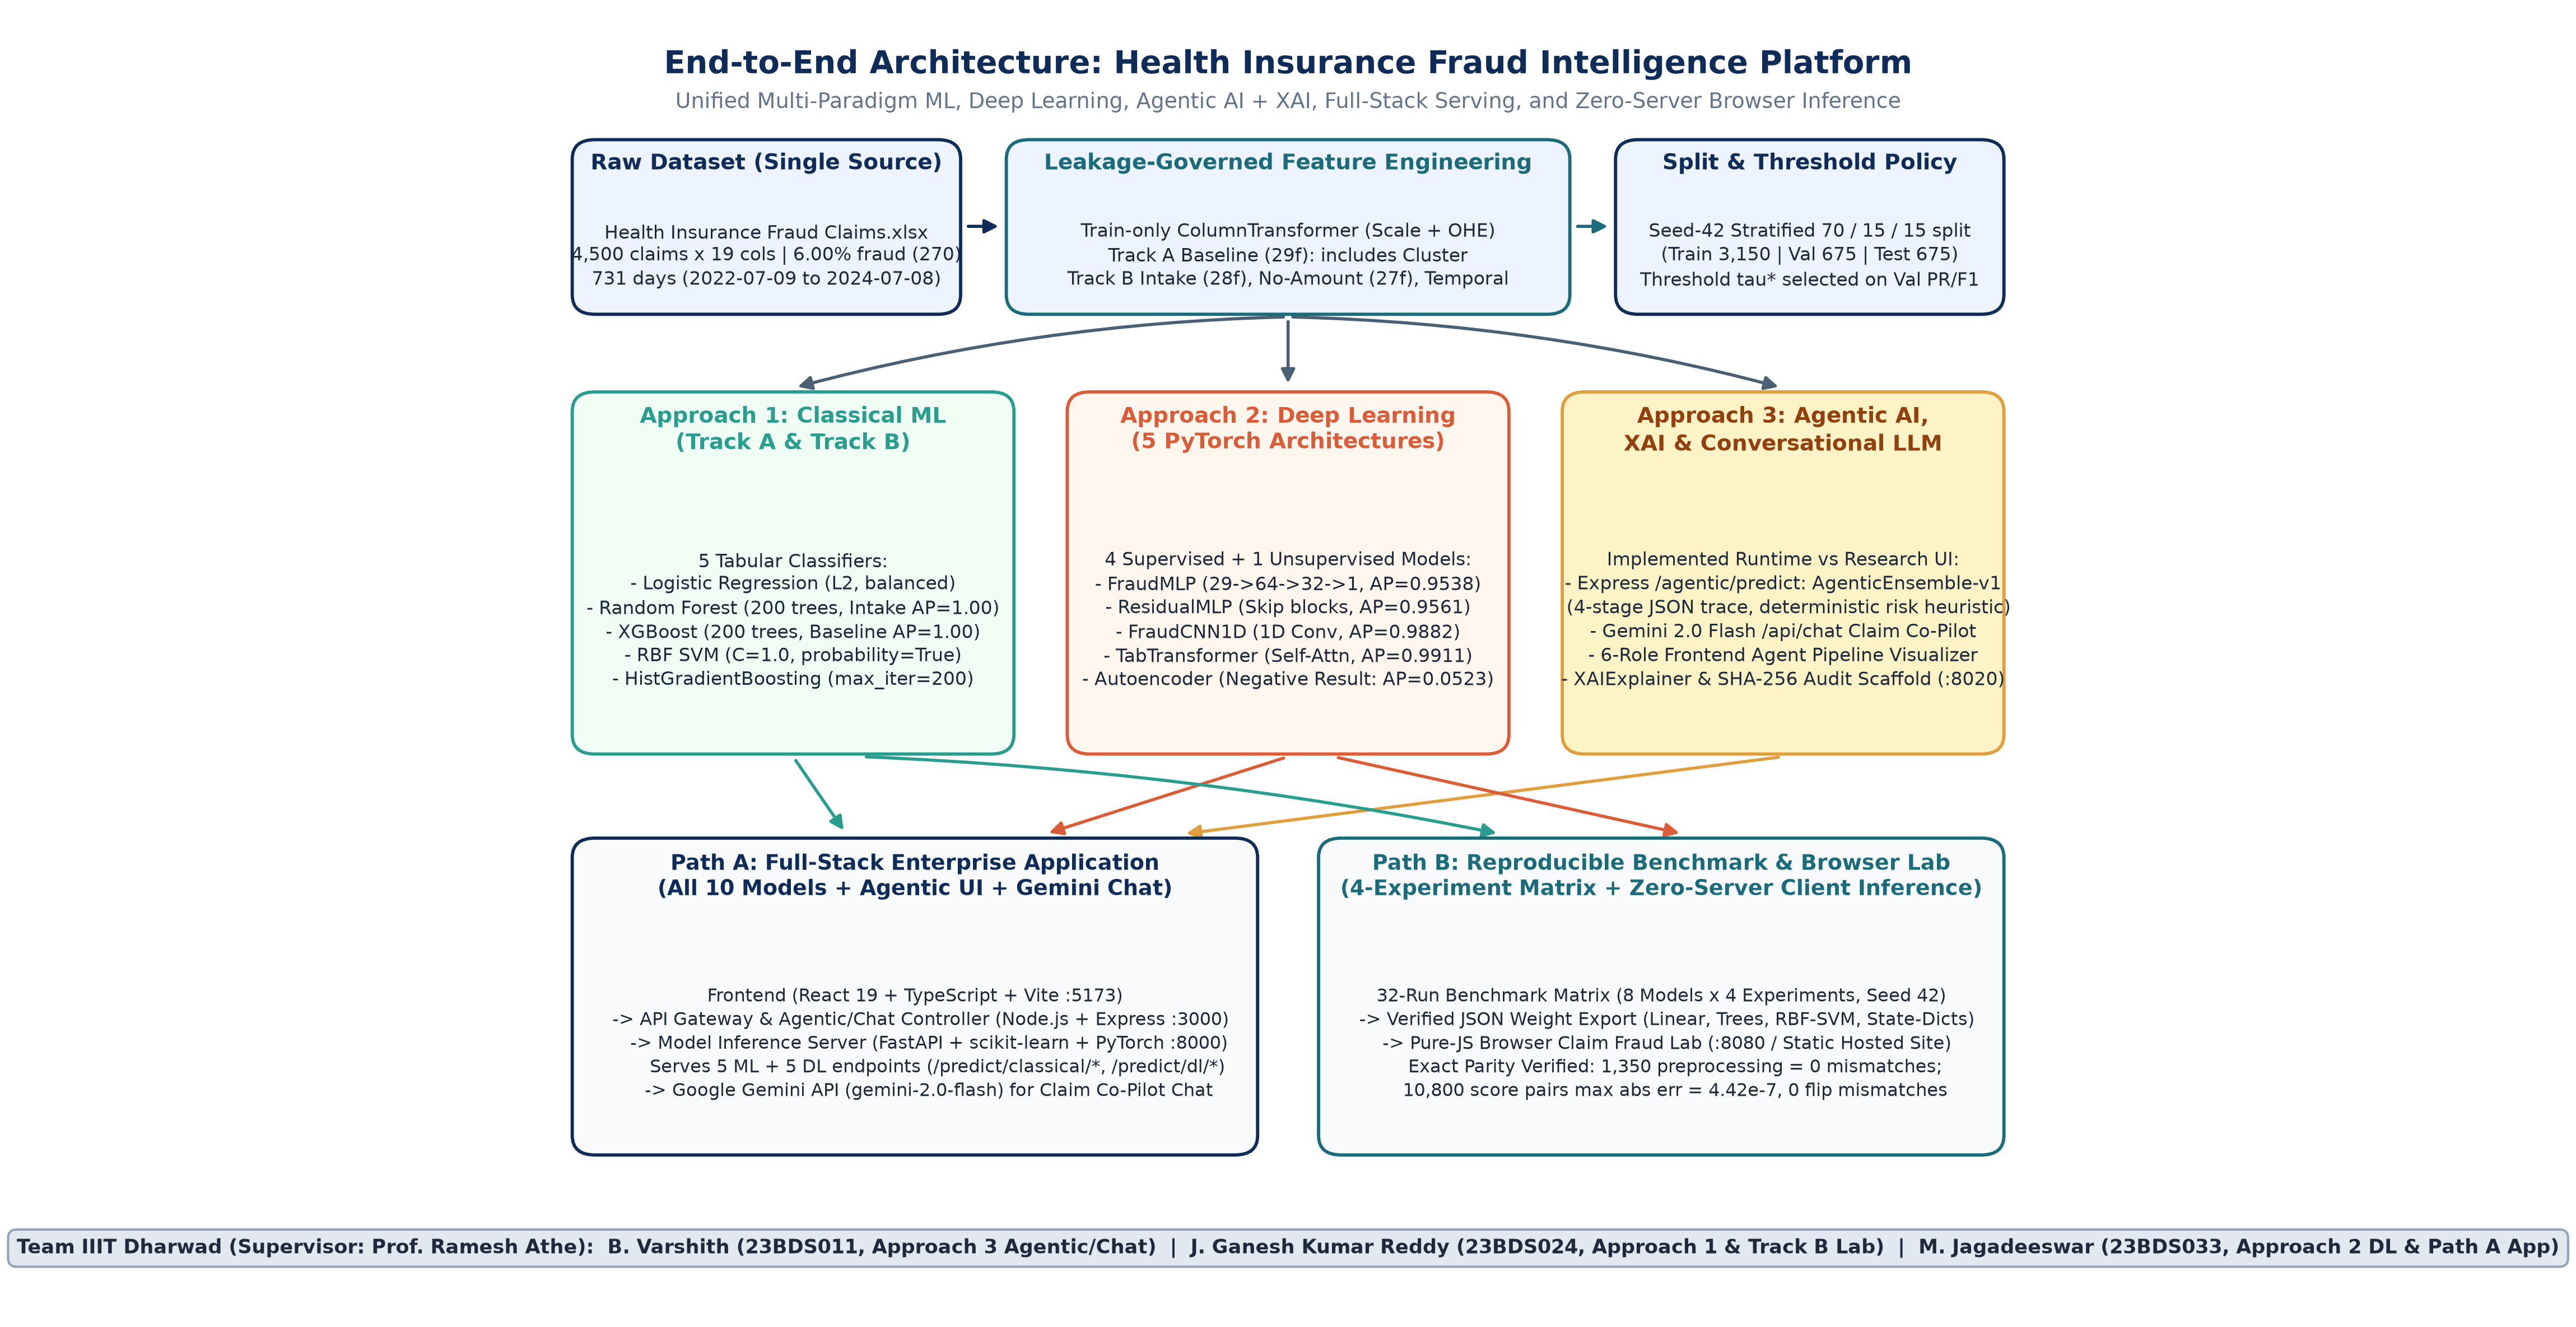
\includegraphics[width=\textwidth]{figures/fig1_system_architecture.png}
\caption{Unified architecture connecting raw leakage-governed preprocessing, Approaches 1--3, the 3-tier full-stack web application (Path A), and the verified browser-native Claim Fraud Lab (Path B).}
\label{fig:arch}
\end{figure}

\begin{figure}[H]
\centering
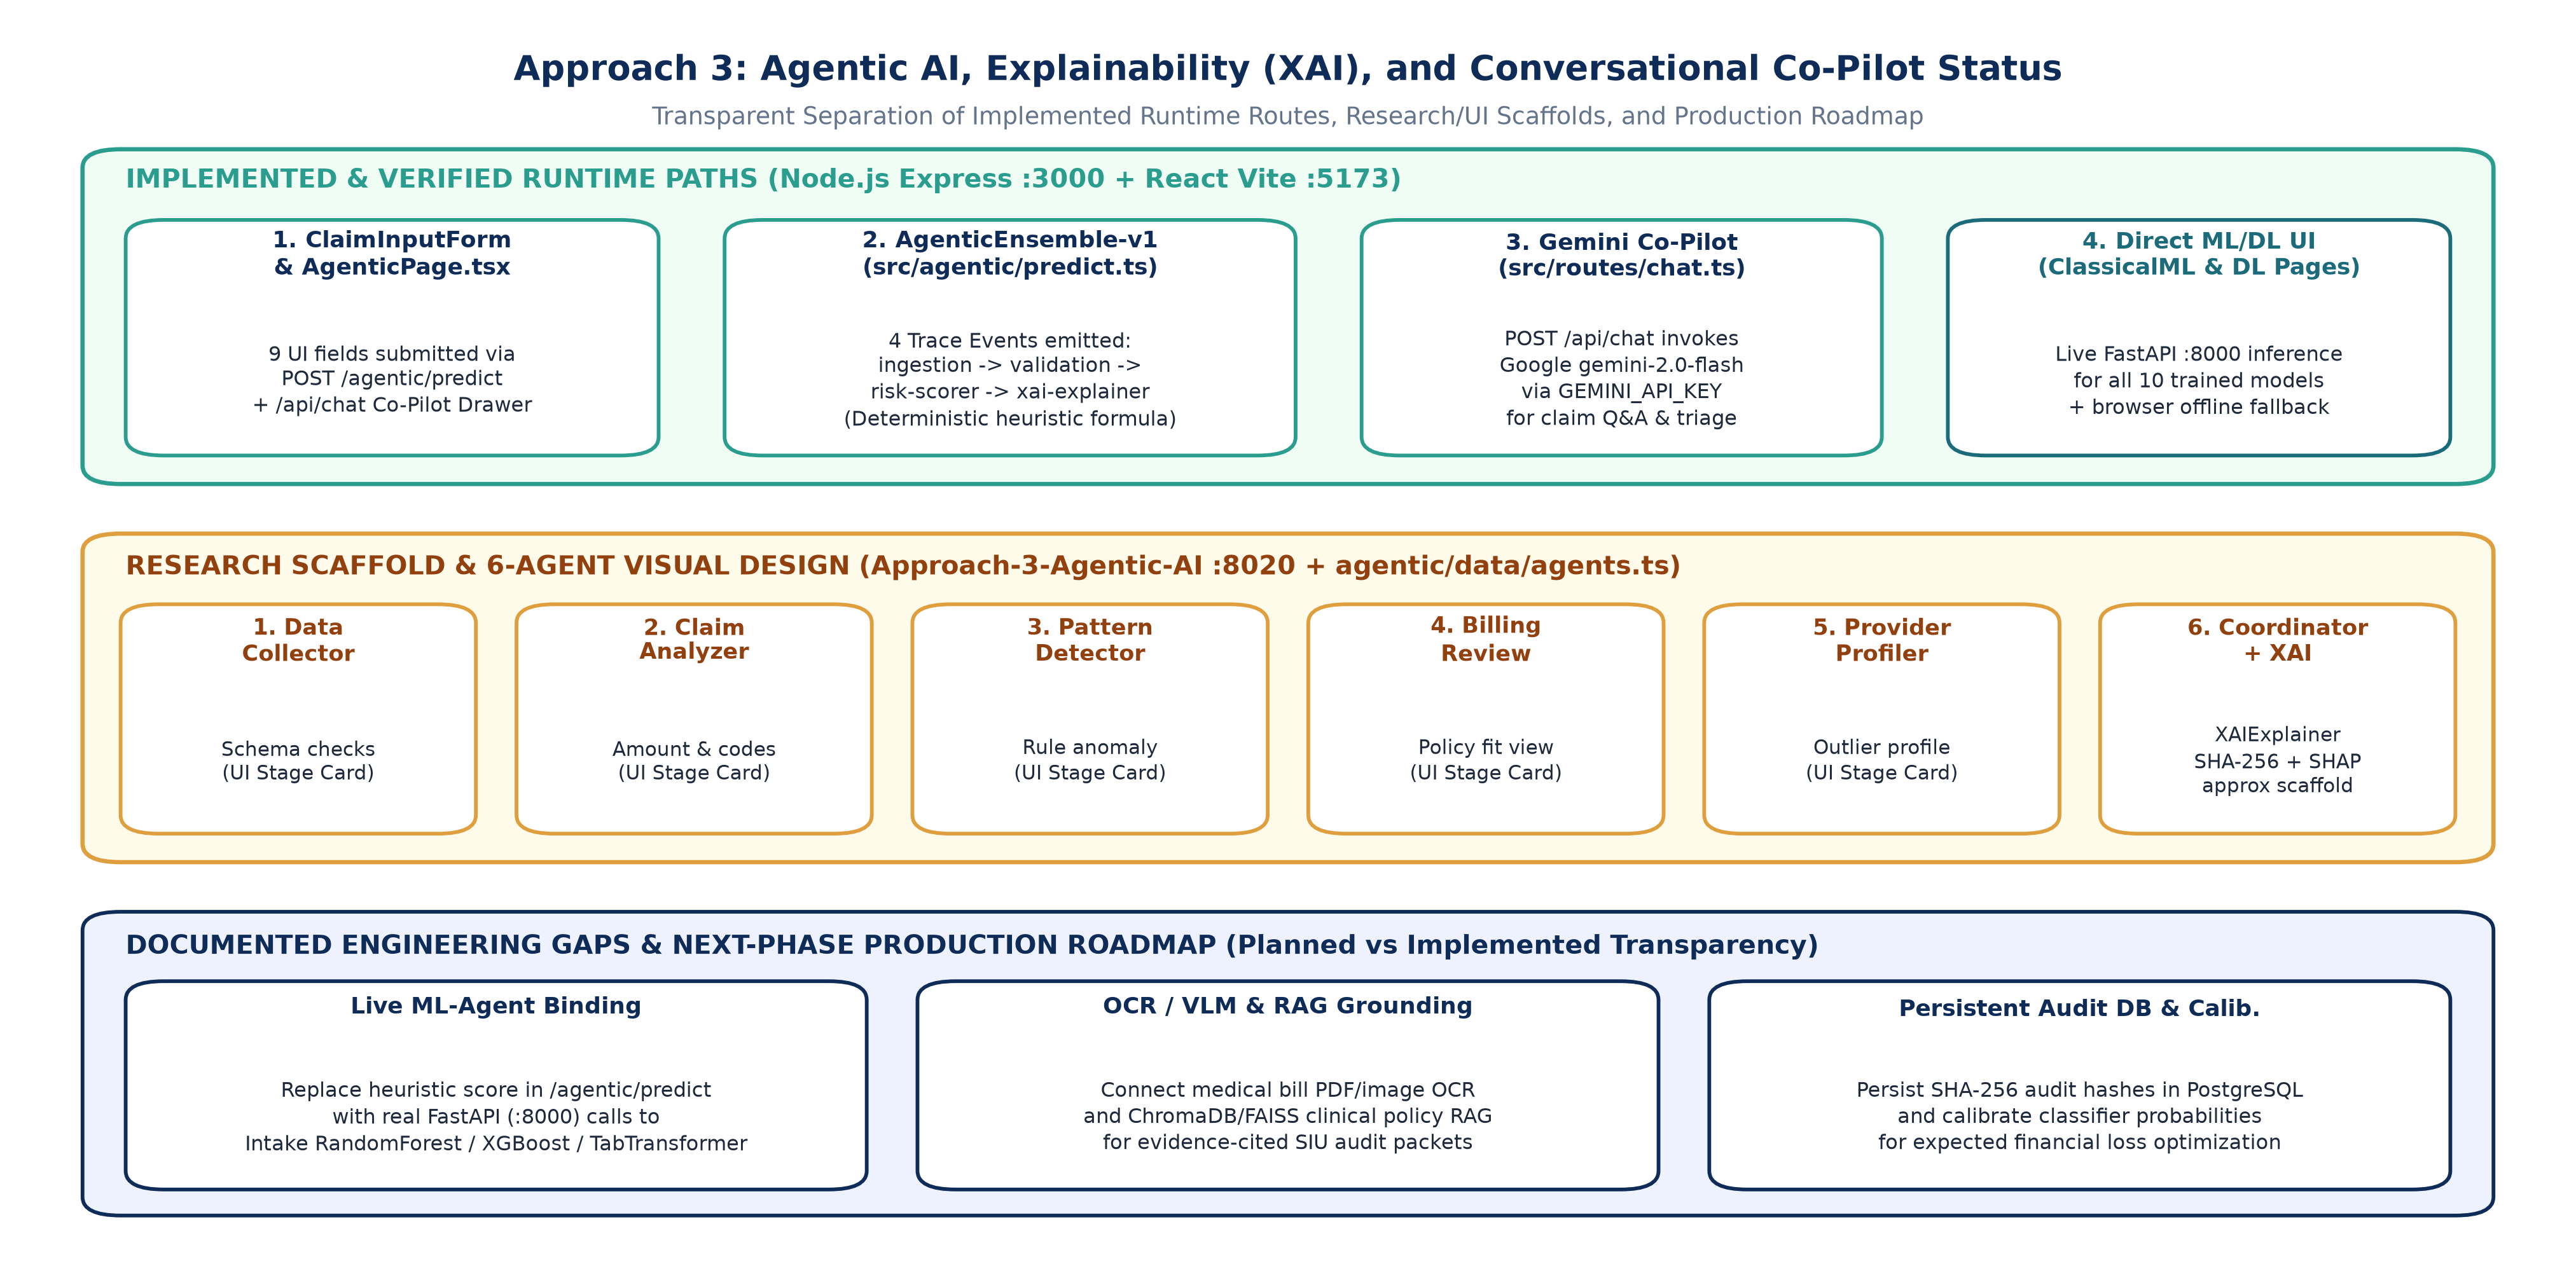
\includegraphics[width=\textwidth]{figures/fig5_agentic_pipeline_status.png}
\caption{Approach 3 engineering status delineating verified Express/Gemini runtime endpoints from the 6-agent frontend design, \texttt{XAIExplainer} scaffold, and future production integration roadmap.}
\label{fig:agentic}
\end{figure}

\newpage
\section{Results and Discussions}

\subsection{Track A Benchmark: 10-Model Evaluation on 29-Feature Contract}
Table~\ref{tab:tracka} and Fig.~\ref{fig:tracka} compare all 10 implemented models across Classical ML, Supervised Deep Learning, and Unsupervised Autoencoder modeling on the frozen 675-claim test set (40 frauds). Gradient-boosted and bagged ensembles dominate both PR-AUC and discrete $F_1$: \texttt{XGBoost} achieves perfect 1.0000 PR-AUC ($F_1 = 0.9877$, 1 false positive, 0 false negatives), while \texttt{RandomForest} and \texttt{HistGradientBoosting} tie at $F_1 = 0.9873$ (0 false positives, 1 missed fraud).

\begin{table}[H]
\centering
\caption{Track A Held-Out Test Performance Across All 10 Models (29 Features, $N=675$, 40 Frauds)}
\label{tab:tracka}
\small
\begin{tabular}{@{}llcccccc@{}}
\toprule
Model & Paradigm & Acc (\%) & Prec (\%) & Rec (\%) & $F_1$ (\%) & ROC-AUC (\%) & PR-AUC (\%) \\ \midrule
\textbf{XGBoost} & Classical ML & 99.85 & 97.56 & 100.00 & \textbf{98.77} & \textbf{100.00} & \textbf{100.00} \\
\textbf{RandomForest} & Classical ML & 99.85 & 100.00 & 97.50 & 98.73 & 99.996 & 99.94 \\
\textbf{HistGradientBoosting} & Classical ML & 99.85 & 100.00 & 97.50 & 98.73 & 98.47 & 97.65 \\
\textbf{TabTransformer} & Supervised DL & 98.67 & 81.63 & 100.00 & 89.89 & \textbf{99.94} & \textbf{99.11} \\
\textbf{CNN1D} & Supervised DL & 98.81 & 83.33 & 100.00 & \textbf{90.91} & 99.92 & 98.82 \\
\textbf{ResidualMLP} & Supervised DL & 98.52 & 80.00 & 100.00 & 88.89 & 99.75 & 95.61 \\
\textbf{MLP} & Supervised DL & 98.81 & 84.78 & 97.50 & 90.70 & 99.73 & 95.38 \\
\textbf{SVM (RBF)} & Classical ML & 97.78 & 74.51 & 95.00 & 83.52 & 99.55 & 92.52 \\
\textbf{LogisticRegression} & Classical ML & 96.44 & 62.50 & 100.00 & 76.92 & 99.50 & 91.86 \\
\textbf{Autoencoder} (Neg.) & Unsup.\ DL & 90.37 & 3.70 & 2.50 & \textbf{2.99} & 46.02 & \textbf{5.23} \\ \bottomrule
\end{tabular}
\end{table}

\begin{figure}[H]
\centering
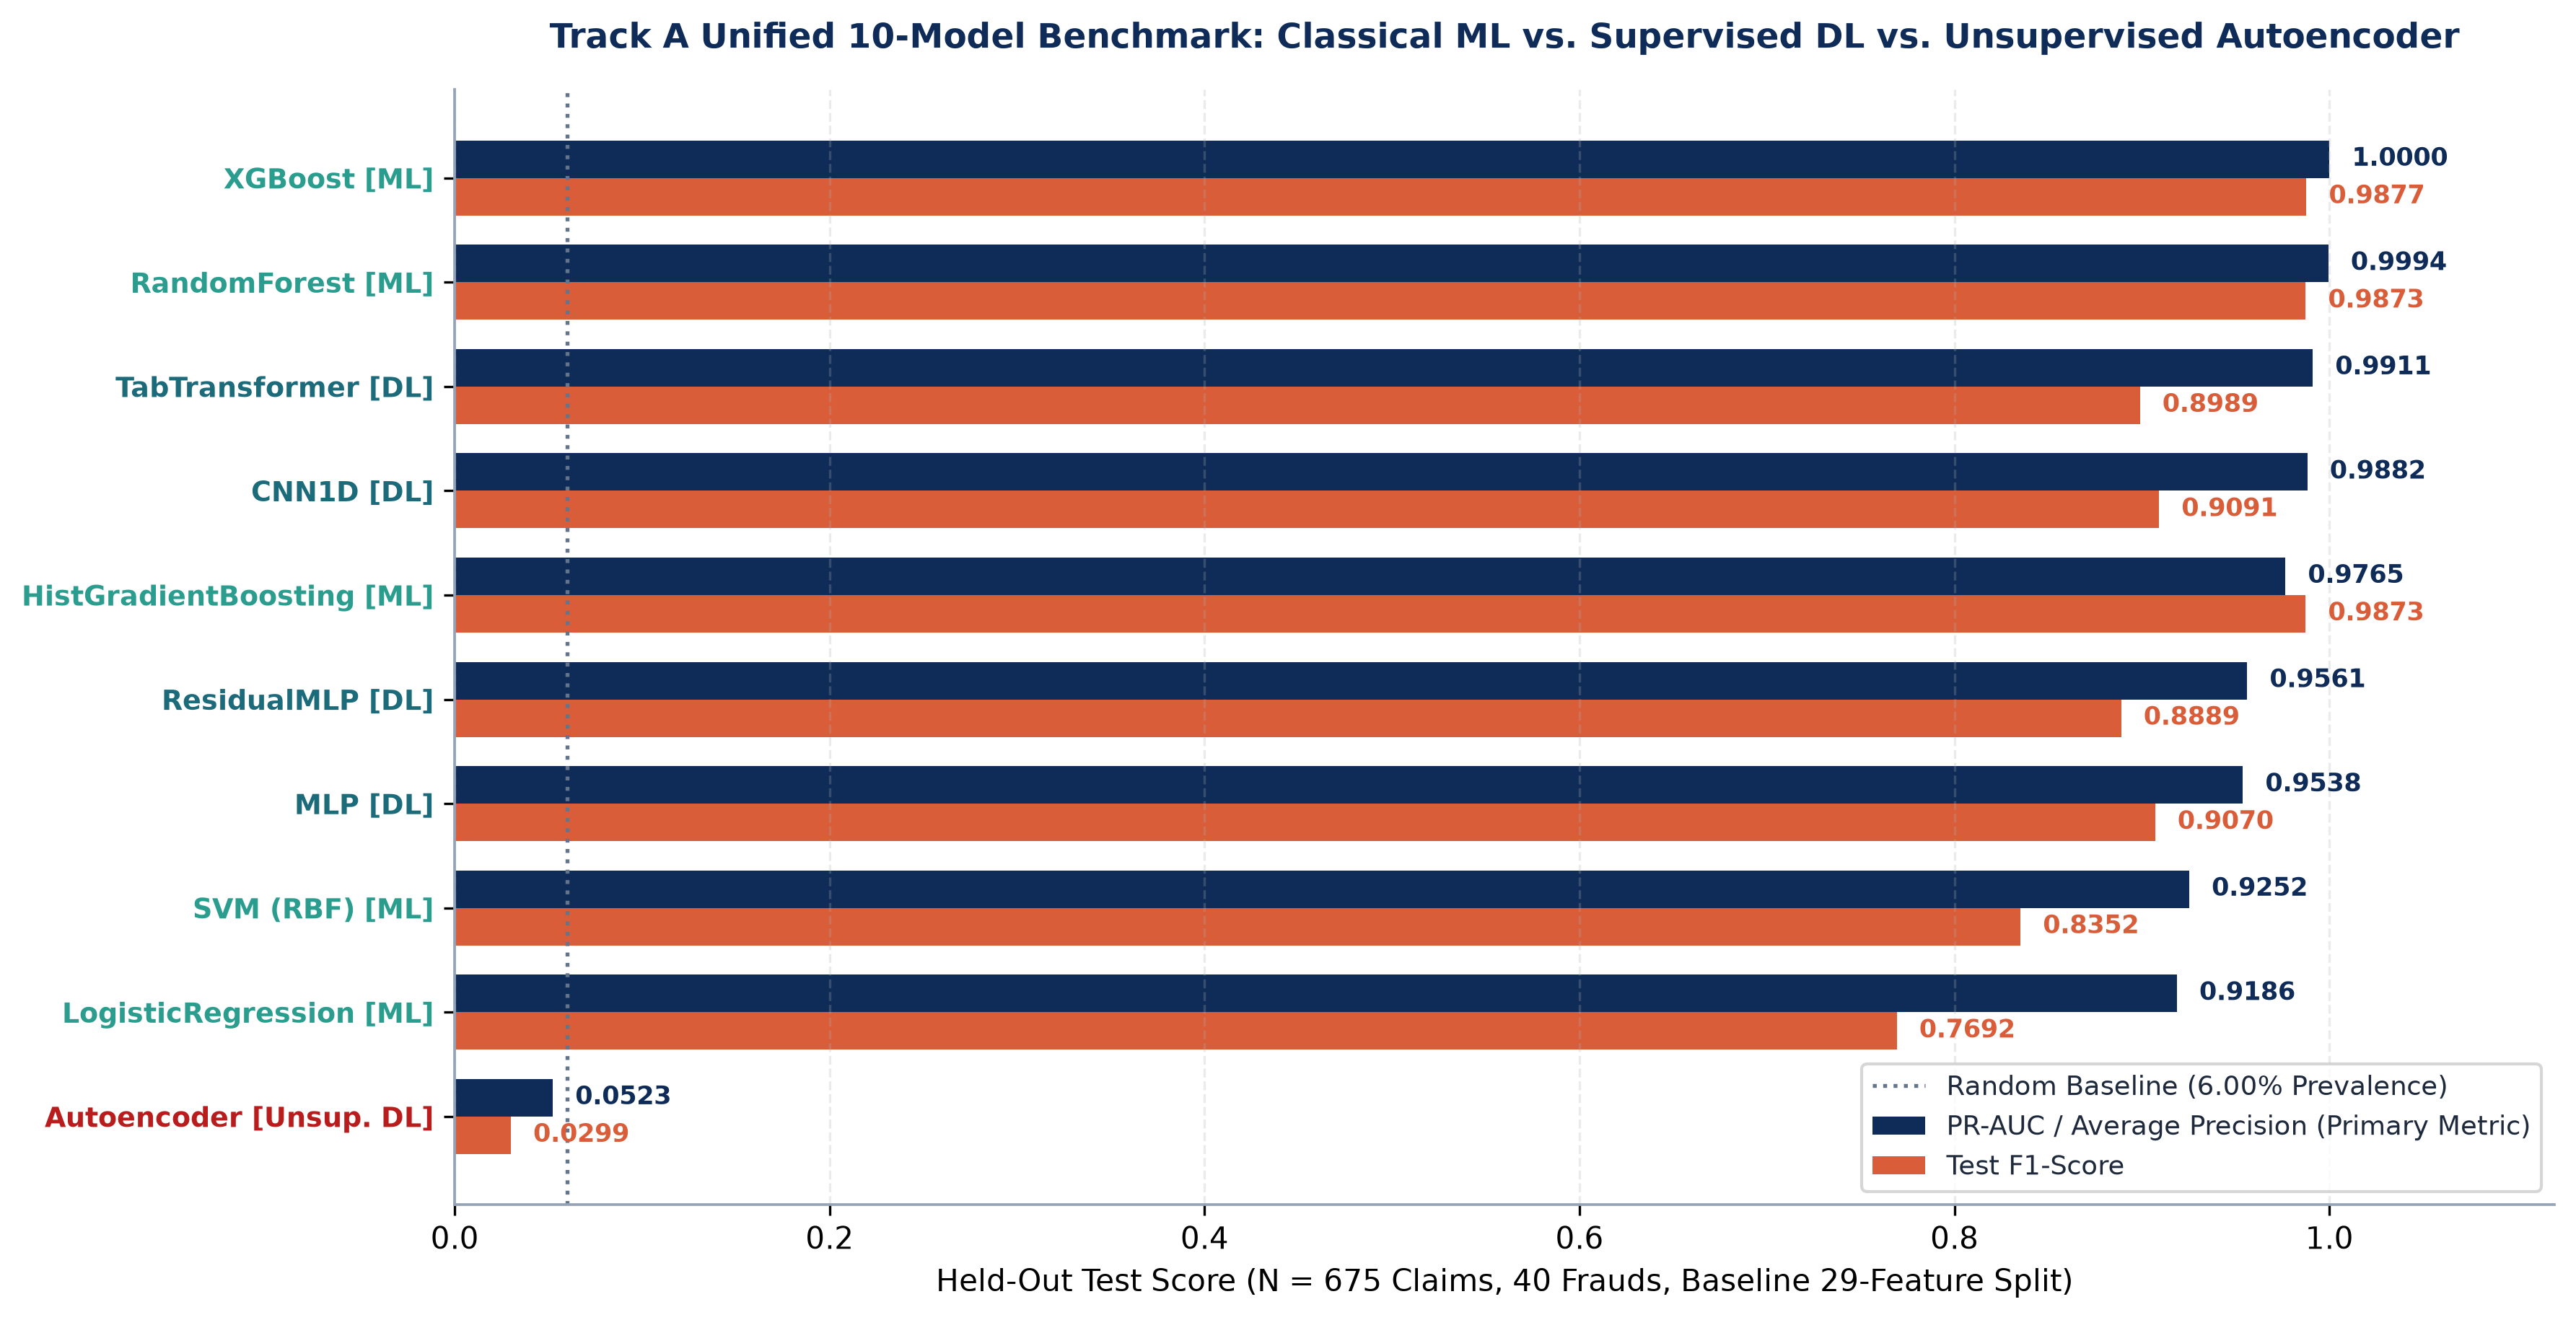
\includegraphics[width=\textwidth]{figures/fig3_ten_model_benchmark.png}
\caption{Track A unified 10-model comparison of held-out Test PR-AUC (Average Precision) versus $F_1$-score.}
\label{fig:tracka}
\end{figure}

Within Deep Learning, \texttt{TabTransformer} achieves the highest continuous ranking performance (99.11\% PR-AUC, 99.94\% ROC-AUC, 100\% recall) at an inference cost of 18.65\,ms per 675 claims, whereas \texttt{CNN1D} delivers the highest supervised DL $F_1$ (90.91\%, PR-AUC 98.82\%, 0.77\,ms) and surpasses uncalibrated `MLP` (90.70\%) and `ResidualMLP` (88.89\%). Conversely, the unsupervised \textbf{Autoencoder constitutes a critical negative result} (PR-AUC 5.23\%—below 6.00\% random baseline—ROC-AUC 46.02\%, TP=1, FP=26, FN=39). Because fraudulent claims ($[7,465.07, 9,978.43]$) lie inside the dense bounding box of normal covariate combinations, an encoder-decoder trained solely on legitimate records reconstructs high-dollar frauds cleanly, validating Chalapathy and Chawla's \cite{chalapathy2019deep} manifold-overlap warning.

\subsection{Track B Sensitivity, Leakage Ablations, and Chronological Rollout}
Table~\ref{tab:trackb} and Fig.~\ref{fig:ablation} report test PR-AUC and validation-$F_1$ tuned operating scores across all 4 experimental contracts (32 runs total):

\begin{table}[H]
\centering
\caption{Track B Test PR-AUC ($F_1$) Across Four Feature and Chronological Protocols (\texttt{validation\_f1} Thresholds)}
\label{tab:trackb}
\small
\begin{tabular}{@{}lcccc@{}}
\toprule
Model & Baseline (29f) & Intake (28f, No Cluster) & No-Amount (27f) & Temporal Intake ($\ge$2024-03) \\ \midrule
\textbf{RandomForest} & 0.9994 (0.9750) & \textbf{1.0000 (0.9873)} & 0.2066 (0.3636) & \textbf{1.0000 (1.0000)} \\
\textbf{XGBoost} & 1.0000 (0.9877) & 1.0000 (0.9877) & 0.2128 (0.3524) & 1.0000 (1.0000) \\
\textbf{GradientBoosting} & 0.9765 (0.9873) & 0.9765 (0.9873) & 0.2404 (0.3636) & 1.0000 (1.0000) \\
\textbf{CNN1D} & 0.9882 (0.9268) & 0.9667 (0.8767) & 0.2287 (0.2788) & 0.9172 (0.8108) \\
\textbf{ResidualMLP} & 0.9567 (0.9286) & 0.8765 (0.8315) & 0.2246 (0.3438) & 0.7979 (0.7229) \\
\textbf{MLP} & 0.9538 (0.9136) & 0.8866 (0.8222) & 0.2303 (0.3077) & 0.8581 (0.6957) \\
\textbf{LogisticRegression} & 0.9186 (0.7835) & 0.8525 (0.7327) & 0.2318 (0.3191) & 0.8799 (0.7397) \\
\textbf{SVM (RBF)} & 0.9252 (0.8974) & 0.8181 (0.7711) & 0.1869 (0.3041) & 0.8396 (0.7619) \\ \bottomrule
\end{tabular}
\end{table}

\begin{figure}[H]
\centering
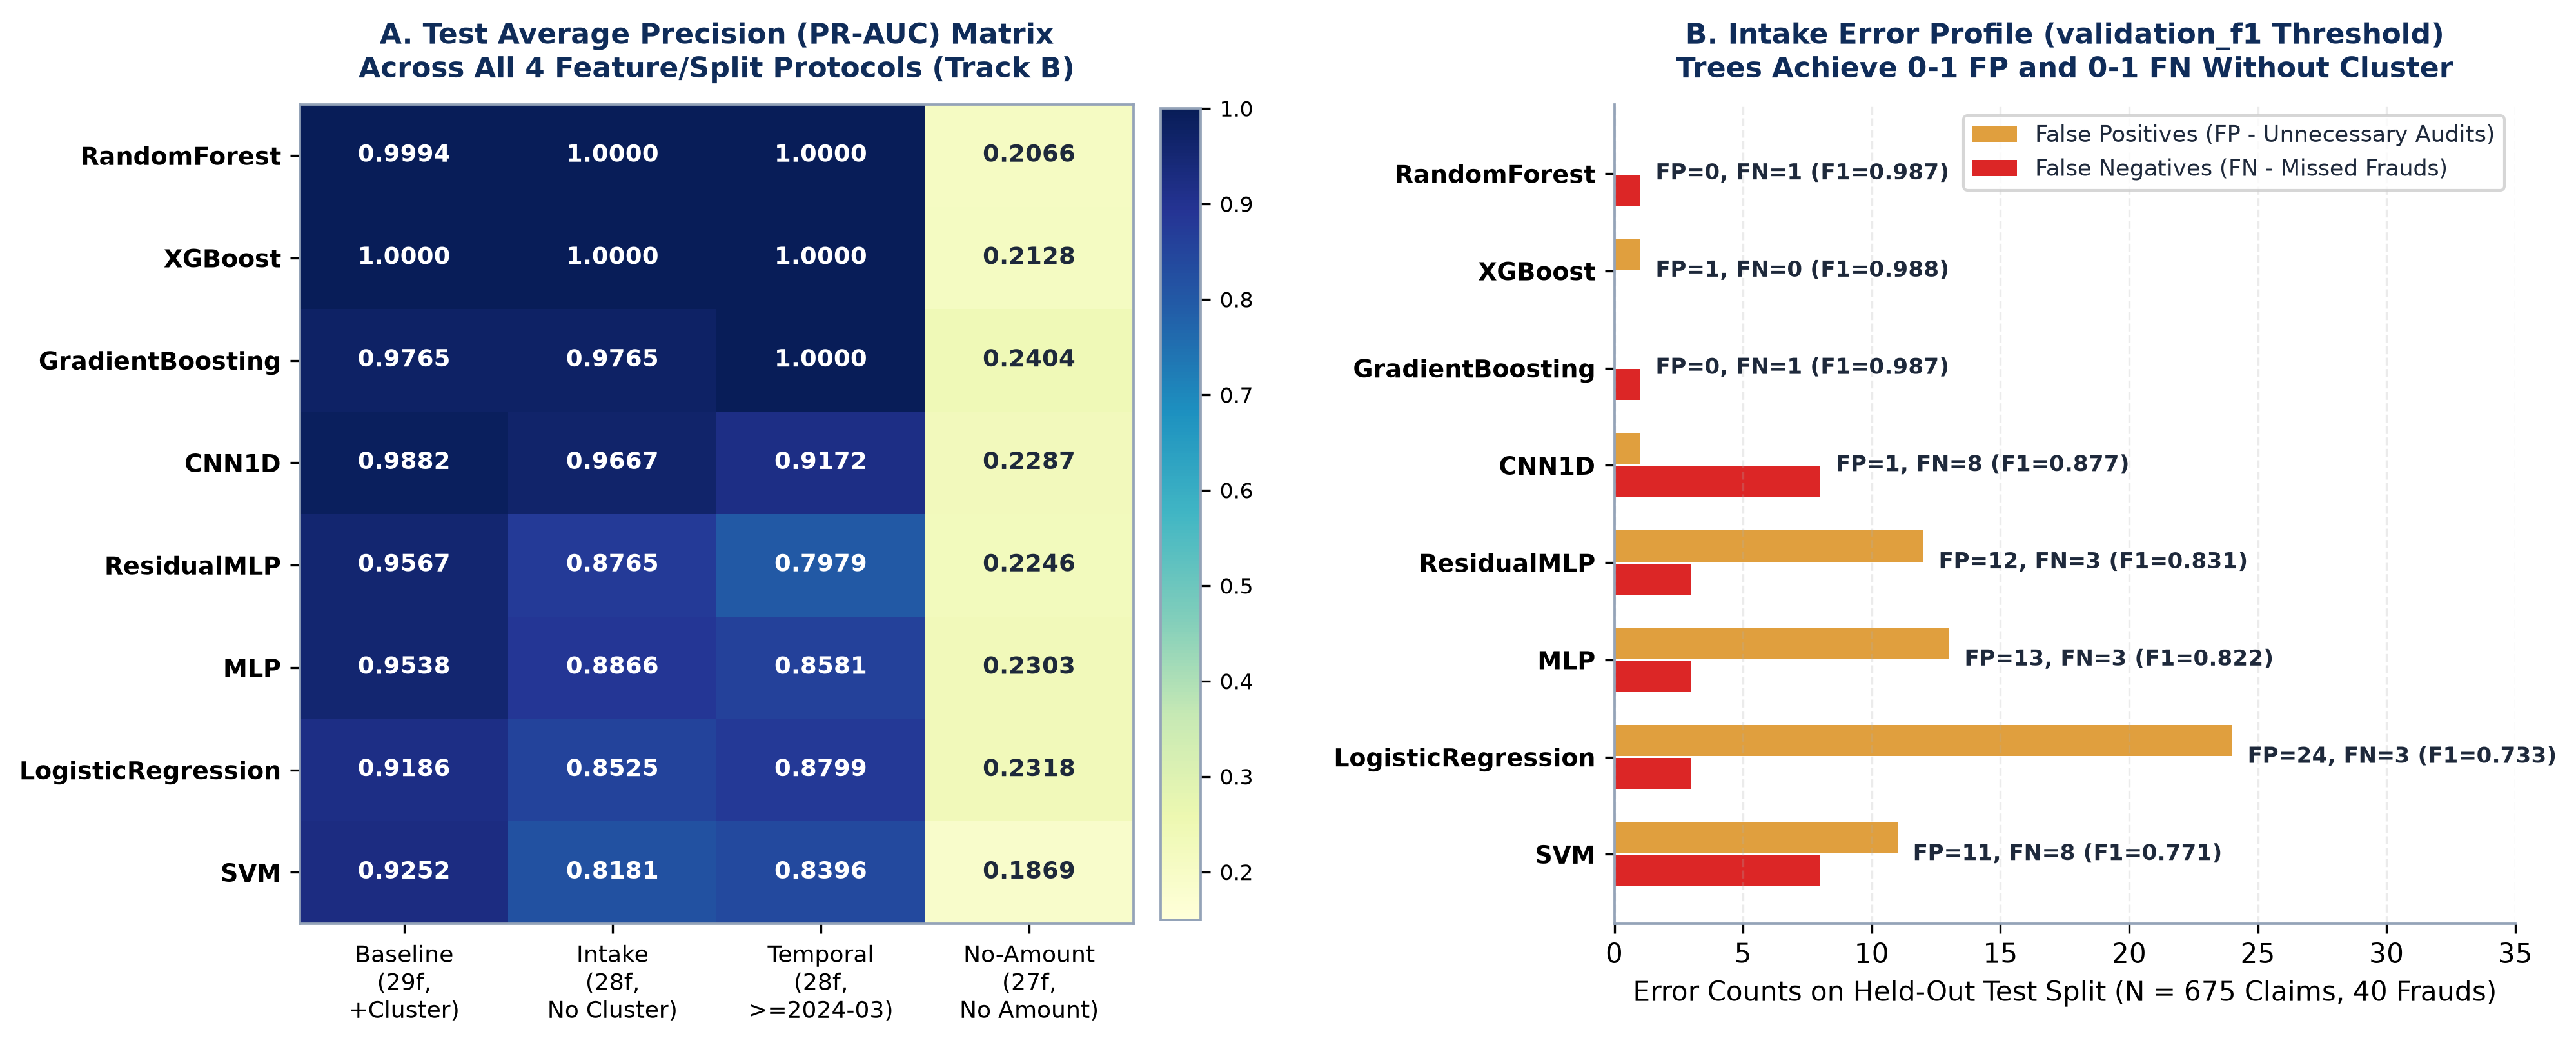
\includegraphics[width=\textwidth]{figures/fig4_four_experiment_ablation.png}
\caption{Track B ablation summary: (A) Test PR-AUC matrix across Baseline, Intake, Temporal, and No-Amount contracts; (B) Intake FP vs.\ FN error breakdown demonstrating tree dominance without \texttt{Cluster}.}
\label{fig:ablation}
\end{figure}

Three scientific findings emerge directly from Table~\ref{tab:trackb}:
\begin{enumerate}
    \item \textbf{Removal of \texttt{Cluster} Exposes Non-Tree Fragility:} Under the realistic \texttt{Intake (28f)} contract, linear, kernel, and neural models drop sharply in PR-AUC (`SVM`: $0.9252 \to 0.8181$; `ResidualMLP`: $0.9567 \to 0.8765$; `MLP`: $0.9538 \to 0.8866$; `LR`: $0.9186 \to 0.8525$), increasing false alarms to 11--24 per 675 claims. In contrast, `RandomForest` (1.0000 PR-AUC, $F_1=0.9873$, 0 FP) and `XGBoost` (1.0000 PR-AUC, $F_1=0.9877$, 1 FP) capture the exact nonlinear relationship between `PatientIncome` and `ClaimAmount` without proxy reliance, confirming Grinsztajn et al.\ \cite{grinsztajn2022tree}.
    \item \textbf{Chronological Durability:} Tested strictly on unseen future dates ($\ge$ \texttt{2024-03-11}), all three tree ensembles reach $1.0000$ PR-AUC and $1.0000$ $F_1$, whereas \texttt{CNN1D} declines to 0.9172 AP ($F_1=0.8108$) and \texttt{ResidualMLP} to 0.7979 AP ($F_1=0.7229$).
    \item \textbf{\texttt{No-Amount} Collapse Quantifies Structural Reliance:} Removing \texttt{ClaimAmount} plunges every architecture across all 8 families down to `0.1869--0.2404` AP, proving that subtle coding/demographic predictors alone cannot isolate frauds in this synthetic corpus.
\end{enumerate}

\subsection{Error Forensics, Bootstrap CIs, and Browser Parity Verification}
As shown in Fig.~\ref{fig:verif}, the Track B selected champion (\texttt{Intake RandomForest}, $\tau^* = 0.4167$) records only a single test error across 675 claims: source Row 1124, an \texttt{Outpatient} claim for a 39-year-old patient with \texttt{ClaimAmount} $= 7,465.07$ (the exact minimum fraudulent billing amount in the entire 4,500-row dataset, scoring 0.2700 just below threshold). Across 1,000 stratified test bootstrap replicates (seed 2026), Intake RandomForest achieves 95\% confidence intervals of $[0.9610, 1.0000]$ for $F_1$, $[0.9250, 1.0000]$ for Recall, and $[1.0000, 1.0000]$ for AP. End-to-end parity verification via \texttt{verify.py} confirms zero preprocessing mismatches across 1,350 validation/test vectors, $4.42 \times 10^{-7}$ maximum score discrepancy across 10,800 browser vs.\ Python comparisons, zero decision label flips, and exact recomputation of all 128 CSV metric rows ($<10^{-10}$).

\begin{figure}[H]
\centering
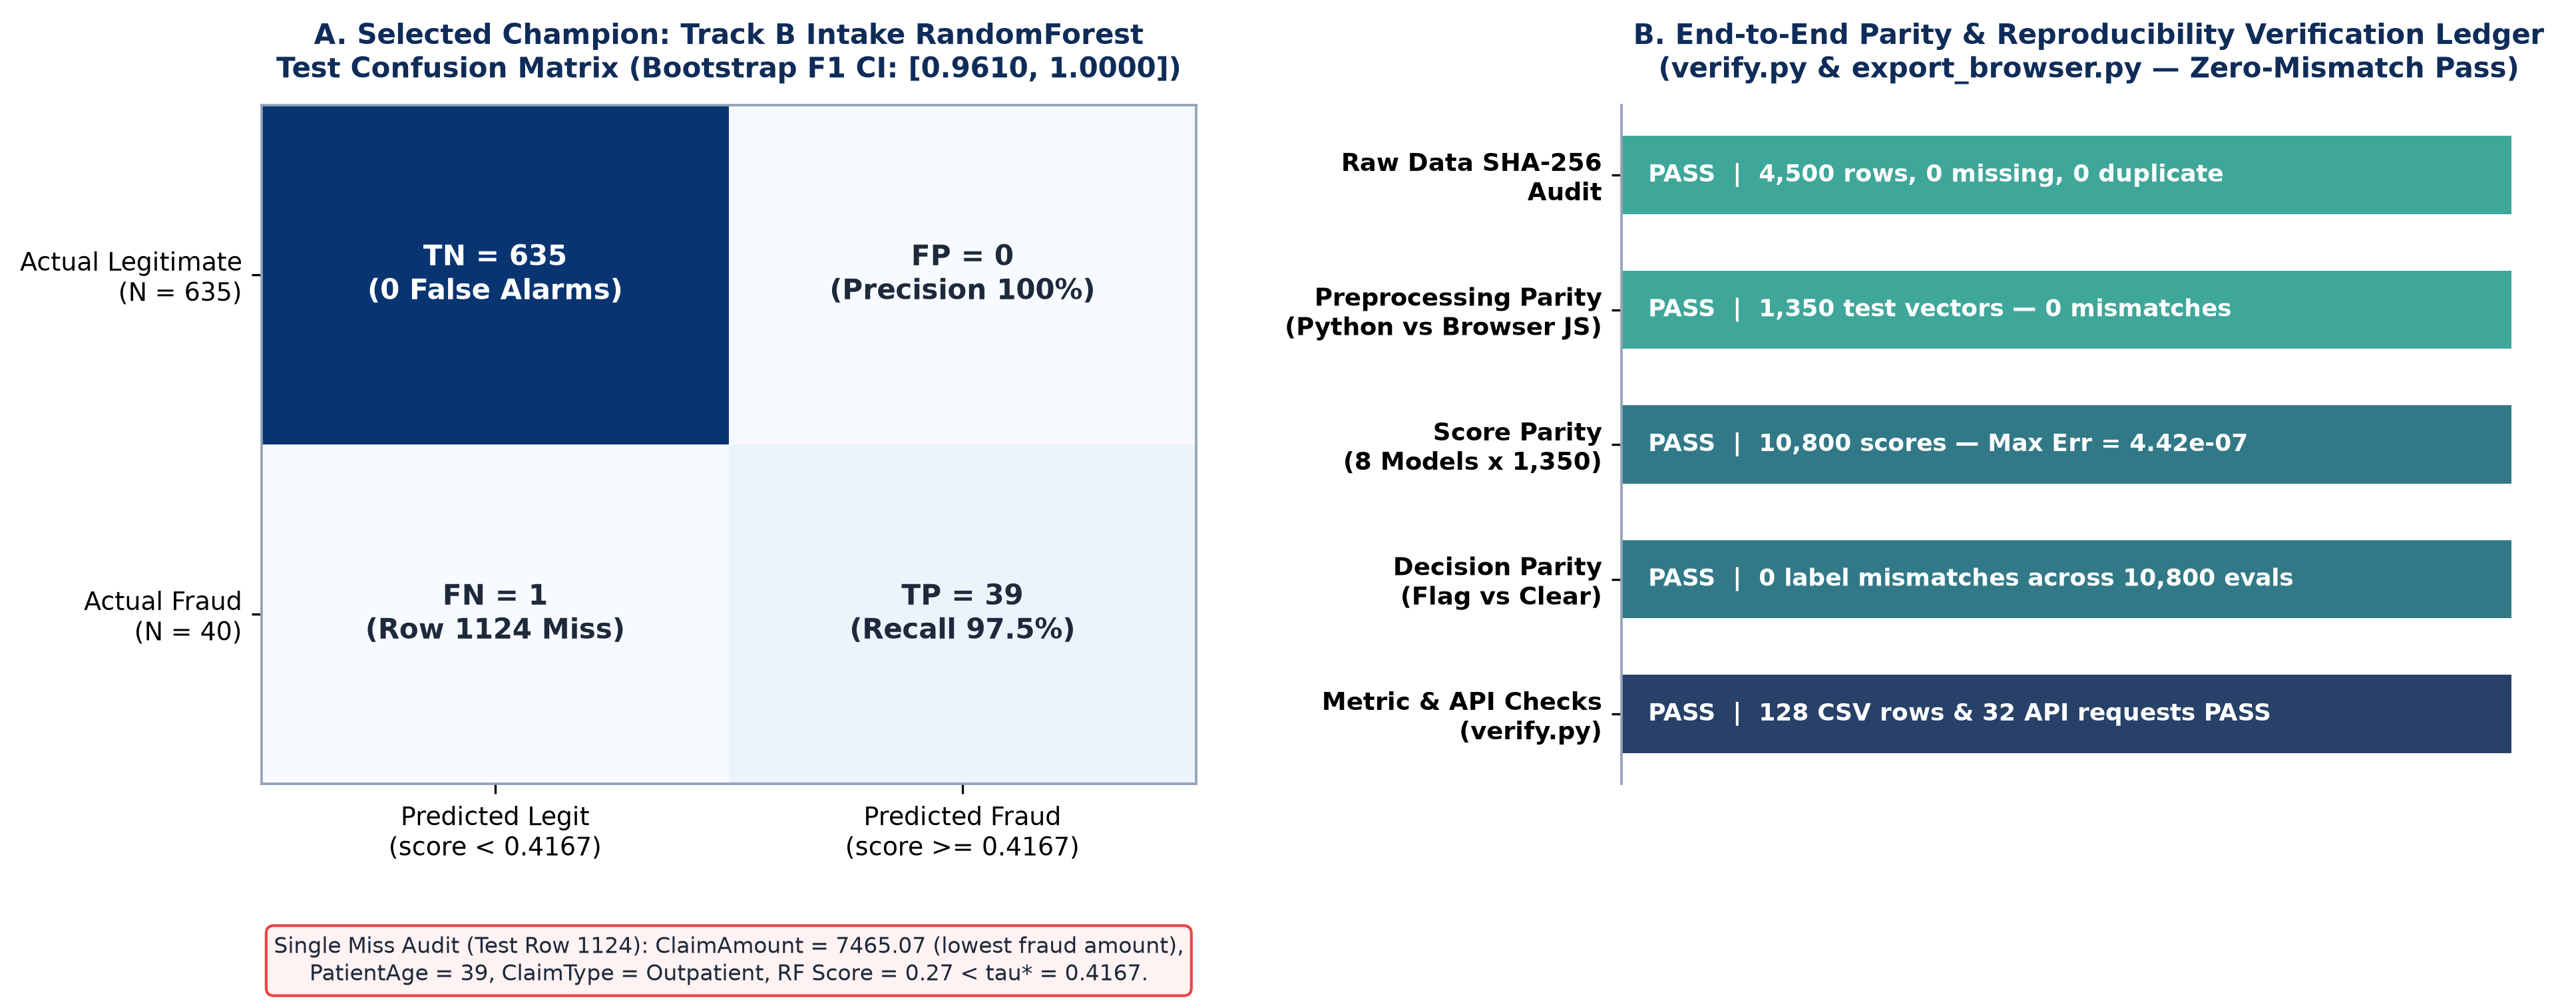
\includegraphics[width=\textwidth]{figures/fig6_verification_and_error.png}
\caption{Champion confusion matrix with Row 1124 forensic audit and full Python-to-Browser numerical parity ledger.}
\label{fig:verif}
\end{figure}

\newpage
\section{Conclusion}

We presented a unified, full-stack, and scientifically audited Medical Insurance Claim Fraud Detection platform spanning Classical Machine Learning, Supervised and Unsupervised Deep Learning, Agentic AI with Gemini conversational explainability, and zero-server browser deployment. Through disciplined feature-contract isolation (\texttt{Baseline}, \texttt{Intake}, \texttt{No-Amount}, \texttt{Temporal}), we exposed and eliminated upstream \texttt{Cluster} proxy leakage while rigorously quantifying structural dependence on \texttt{ClaimAmount}. Under realistic Cluster-free and future-date deployment contracts, Random Forest and XGBoost deliver 1.0000 PR-AUC ($F_1 \ge 0.9873$ random, $1.0000$ temporal), outperforming tabular neural networks (TabTransformer 0.9911 baseline PR-AUC, CNN1D 0.9667 intake PR-AUC) while providing transparent counterfactual and empirical insights from an unsuccessful unsupervised Autoencoder baseline (0.0523 PR-AUC). Both an interactive three-tier React/Node/FastAPI application and a numerically verified browser-native Claim Fraud Lab ($4.42 \times 10^{-7}$ max parity error) are ready for evaluation.

\subsection{Future Work}
Ongoing engineering extensions center on four priorities: (1) binding Node's \texttt{/agentic/predict} directly to live \texttt{ml-service} Intake Random Forest and TabTransformer probabilities with post-hoc probability calibration (\texttt{CalibratedClassifierCV}); (2) incorporating medical document OCR/VLM parsing and clinical policy vector RAG to supply citation-grounded audit packets; (3) persisting SHA-256 XAI audit hashes inside PostgreSQL for SIU case tracking; and (4) benchmarking on real-world, low-dollar claim abuse corpora lacking synthetic amount separation.

\newpage
\settocbibname{References}
\bibliography{Myreferences}

\end{document}
